\documentclass[11pt]{article}
\setlength{\parskip}{1.5em}
\usepackage[authoryear]{natbib}
\usepackage{graphicx}
\usepackage{float}
\graphicspath{ {./results/} }
\title{Model Fitting for Bacterial Population Growth Data}
\author{An Nguyen}

\begin{document}

\begin{titlepage}

        \centering
		\vspace*{2cm}
		\Large
		\emph{MSc Computational Methods in Ecology and Evolution}\\
		\vspace*{1cm}
		\Large
		\textbf{CMEE Mini Project}\\
		
		\vspace*{3cm}
		\Huge
		\textbf{Model Fitting for Bacterial Population Growth Data}\\
		
		\vspace{3cm}
		\Large
		
		\textbf{Author:} An Nguyen \textit{(an.nguyen21@imperial.ac.uk)}\\
		\vspace*{1cm}
		\textbf{Word Count:} 1795

	\end{titlepage}
\newpage
\tableofcontents
\newpage
\addcontentsline{toc}{section}{Abstract}
\section*{Abstract}
Model fitting is used to describe the trend of a series of data points.  The aim of this project is to identify a model which best represents the provided bacterial growth data. I selected one linear function and three different sigmoidal functions to fit the growth curve of various bacterial species. They are the linear growth mode, classical mechanistic model, modifed Gompertz model and Baranyi model. My goal is to compare the three and then select the best fitting model. The best fitted model was chosen through comparison of the Akaike Information Criterion. Out of the four models, the classical mechanistic model was the best fitting for this data set. 

\newpage
\section{Introduction}

Bacterial growth follows three distinct phases: lag phase, exponential phase, and finally stationary phase. During the lag phase, bacteria prepare for growth and nutrient uptake by activating the necessary transcriptional machinery. This preparation leads to rapid bacterial growth in the exponential phase, population grows to be twice of the previous generation. Once resources are used up by the growing population and carrying capacity is reached, the growth declines and the growth rate enters the stationary phase. In this project, the bacterial growth rate was recorded against time. My goal is to choose the best fitting sigmoidal growth curve for this data set. 

Different non-linear regression models have been developed for fitting bacterial growth, the three models tested in this project are classical mechanistic model (\cite{verhulst1838notice}), modifed Gompertz model (\cite{PMID:16348228}) and Baranyi model (\cite{BARANYI1994277}). Non-linear regression is chosen instead of linear regression because the relationship of bacterial growth over time is not linear. These models have been widely used in literature for bacterial growth prediction. In these models, bacteria are considered to be homogeneous and their growth is uniform. The data are also fitted to a one-phase linear exponential growth model. Details for each of the models are as follows:

1. Linear exponential growth model
\begin{equation}
    N_{t} = at + N_{0}
\end{equation}
\emph{N\textsubscript{t}} is the population at time t. a is the rate of population change over time. \emph{N\textsubscript{0}} is the population size at time 0. This model does not represent the typical bacterial growth curve as there is no lag phase or stationary phase, it is only used to estimate certain model parameters. 

2. Classical mechanistic model

\begin{equation}
    N_{t} = \frac{N_{0} N_{max}  e^{r_{max}(t)}} {N_{max} + N_{0}  (e^{r_{max}(t)} - 1)}
\end{equation}
This model is also known as the Logistic (Verhulst) model. \emph{N\textsubscript{t}} represents the population at time t.  \emph{N\textsubscript{0}} stands for initial population size,  \emph{N\textsubscript{max}} is the carrying capacity of that population, also denoted as \emph{K}. \emph{r\textsubscript{max}} is the maximum growth rate. 

3. Modified Gompertz model:

\begin{equation}
    N_{t} = N_{0}(\frac{N_{max}}{N_{0}}) ^ {e ^ {-e ^ {\frac{e ^1 r_{max}(t_{lag} - t)}{log\frac{N_{max}}{N_{0}}} + 1}}}
\end{equation}
The Gompertz curve has been used to describe change over a time series. It has been modified by \cite{PMID:16348228} to illustrate population growth. \emph{N\textsubscript{t}}, \emph{N\textsubscript{0}} carry the same meaning as the classical mechanistic model. For the modified Gompertz, the maximum growth rate \emph{r\textsubscript{max}} is the tangent of the inflection point on the curve, and the \emph{t\textsubscript{lag}} is duration of the lag phase, demonstrated on the curve as the x-intercept of the tangent line. 

4. Baranyi model:
\begin{equation}
    N_{t} = N_{0} + r_{max}At - log(1 + \frac{{e ^ {r_{max}A} - 1}}{e^{N_{max} - N_{0}}})
\end{equation}
where:
\begin{equation}
    At = t + \frac{1}{r_{max}}log({e ^ {-r_{max}t_{lag}} + e ^ {-h} - e ^ {-r_{max} * t - h}})
\end{equation}
\begin{equation}
    h = r_{max} t_{lag}
\end{equation}
The Baranyi function has the same parameter as the modified Gompertz model with \emph{h} as an additional parameter. \emph{h} represents the initial physiological state of the organism which has influences on the lag phase. Over the years, Baranyi model seems to be more favoured over the modified Gompertz model as the additional parameter \emph{h} helps separate the effects of the initial environment from the effects of the current physiological state. 

Goodness of fit of each model is determined through the Akaike Information Criterion (AIC) (\cite{1100705}). AIC is good for both nested and non-nested models; it also follows the Parsimonious rule in model fitting and rewards model with less parameters. This helps with picking a model that neither under-fits nor over-fits. The assumption for AIC is the more information a model retains, the better its quality. On its own, the raw AIC is meaningless. Therefore, for assessment of the model candidates, I use the delta AIC ($\Delta$AIC) and Aikaike weights ({AIC\textsubscript{w}}) ({\cite{doi:https://doi.org/10.1002/9781118856406.app5}}). $\Delta$AIC is the difference between the lowest AIC ({min\textsubscript{$\Delta$AIC}}) and the AIC of the compared model. The best model has $\Delta$AIC equals to 0. {AIC\textsubscript{w}} are obtained through the relative likelihood values, they are calculated by dividing the candidate's $\Delta$AIC by the sum of the $\Delta$AIC for all candidates. The {AIC\textsubscript{w}} represents the probability of that model being the best, for example, if the {AIC\textsubscript{w}} equals to 1, it means the candidate has a 100\% probability of being the best fitting model. In other words, the closer the {AIC\textsubscript{w}} is to 1, the better the model. 

One disadvantage of the classical mechanistic model, Gompertz model, and the Baranyi model is that they do not take into account dying bacteria and cells, in other word, negative growth curve ({\cite{doi:10.1080/10408398.2011.570463}}), therefore the data need to be cleaned up and any data point that does not satisfy the positive growth rate requirement would be removed. 

\newpage
\section{Methods}
\subsection{Computing Tools}
\emph{Python version 3.8.10} was used for data wrangling and clean up any unwanted data points. The packages Panda and Numpy were loaded to help with this step. 

\emph{R version 4.1.2} was used for calculating the initial parameters, carrying out model fitting and analysis. The package minipack.lm, function nlsLM() was used to fit non-linear regression models. Package qpcR, function akaike.weights() was used to calculate the $\Delta$AIC and {AIC\textsubscript{w}}. Package dplyr was used to manipulate data in the data frame. 

\emph{Bash} was used to run all the Python and R scripts. The latex file was also included in the bash script to produce this report.  

\subsection{Data Preparation}
The data set provided contained multiple information about different bacterial species. I created a unique ID for each of them by combining the "Medium", "Temp" and "Citation" columns. As these unique IDs were quite long, I converted them to numeric ID. I also filtered the data set to only include three columns which are "ID", "PopBio" and "Time". Any value less than 0 in "Time" and "PopBio" was also removed as it is not biologically possible to have negative time and the chosen models are not suitable for negative growth data. Any species with less than 5 data point was also excluded as 5 is the minimum number of data points required. Data in "PopBio" was also converted to natural logarithm.  Finally, the wrangled data were exported to a csv file. The number of population fit for analysis was 275.

\subsection{Model Fitting and Selection}
First step to non-linear regression model fitting is finding the starting value for the five parameters \emph{t}, \emph{N\textsubscript{0}}, \emph{N\textsubscript{max}}, \emph{r\textsubscript{max}}, \emph{t\textsubscript{lag}}. The linear growth does not require starting values as it is a linear model. The classical mechanistic model require starting values for \emph{t}, \emph{N\textsubscript{0}}, \emph{N\textsubscript{max}}, \emph{r\textsubscript{max}}, Gompertz and Baranyi models require the same parameters with the addition of \emph{t\textsubscript{lag}}.  \emph{t} was taken from the wrangled data file, \emph{N\textsubscript{0}} is the initial population size, in other words, the minimum data point of that population, \emph{N\textsubscript{max}} is the carrying capacity, or the maximum data point of the population. \emph{r\textsubscript{max}} is the maximum growth rate, I attempted fitting the data to a linear regression model and use the slope of the straight line as the starting point for \emph{r\textsubscript{max}}. For any calculated \emph{r\textsubscript{max}} that was less than 0, the data set that \emph{r\textsubscript{max}} belonged to was removed. After this step, the number of data sets dropped to 269. The last time point before the growth curve entered exponential phase \emph{t\textsubscript{lag}} was calculated by taking the second derivative of the natural logarithm of "PopBio". Values of \emph{t\textsubscript{lag}} was also checked to see if there was any negative value. As there was none, the number of data sets for model fitting remained at 269. 

Once the initial starting values for the parameters had been obtained, I applied the function nlsLM() from the R package minpack.lm to the data and their starting values. nlsLM() is used for non-linear regression fitting for classical mechanistic model, Gompertz model, and Baranyi model; as the linear growth model is a linear regression model, the function lm() was used instead. 

AIC values were calculated for each model. The $\Delta$AIC was found by determining the lowest AIC value. Normally, to get the $\Delta$AIC, one has to go through another step of subtracting the lowest AIC from the AIC value of that model. Here, I took a shortcut by finding the lowest AIC and used that for model selection. This is because the best model has $\Delta$AIC equals to 0, in other words, $AIC - {min\textsubscript{$\Delta$AIC}} = 0$, which means the model with the lowest AIC will have its $\Delta$AIC equals to 0. {AIC\textsubscript{w}} was computed using the qpcR package, akaike.weights() function. The model with the lowest AIC and the highest {AIC\textsubscript{w}} was selected as the best model.
\newpage
\section{Results}
Data wrangling resulted in 285 unique data sets. As some initial values for the \emph{r\textsubscript{max}} was negtive, those data sets were excluded from model fitting, resulting in 269 sets. Each set had their own plot showing which models fit the data. 

Out of all four models, the linear growth model managed to fit the most data (269 fits), followed by the classical mechanistic model (241 fits), Gompertz (146 hits), and Baranyi (82 hits) (Figure 1).

\begin{figure}[H]
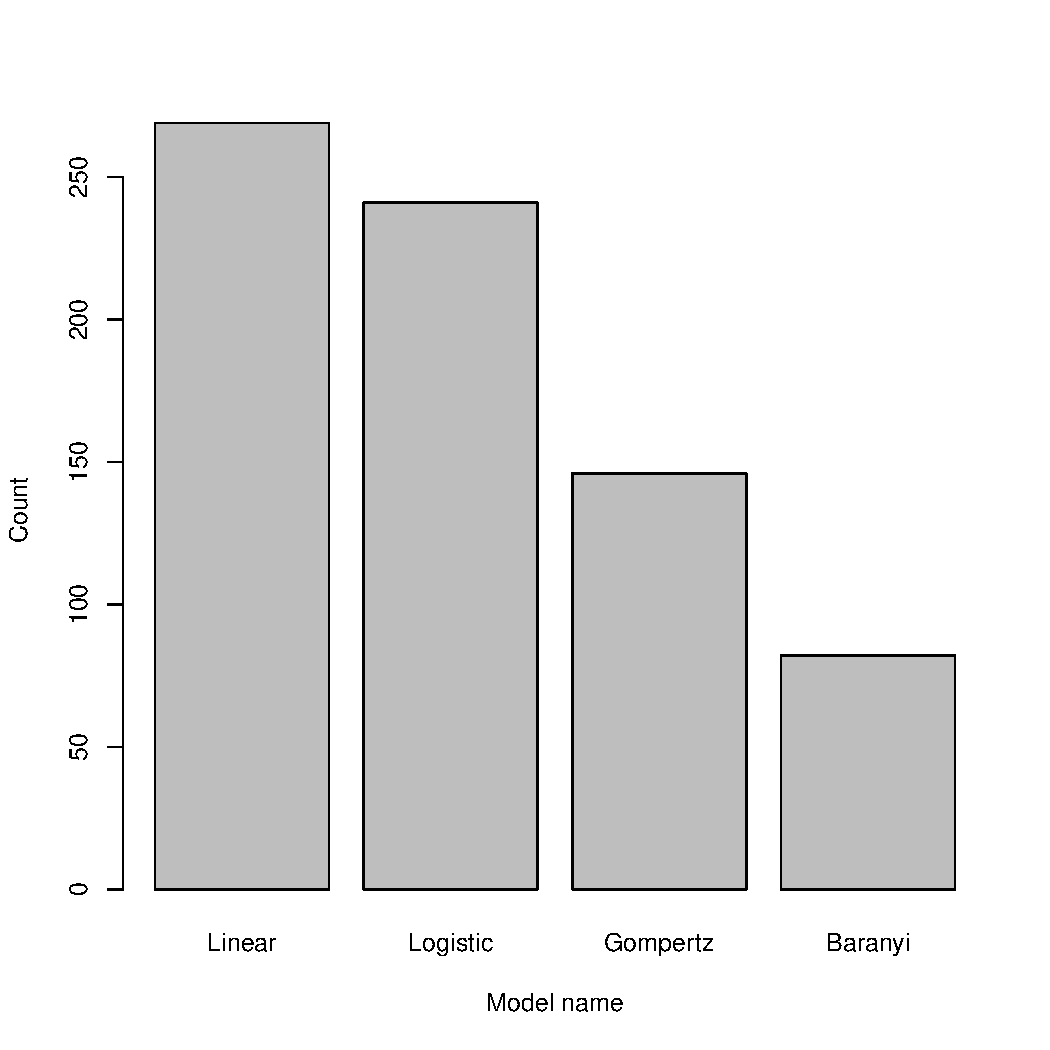
\includegraphics[keepaspectratio, width = 5in, height = 4in]{../results/numfit.pdf}
\centering
\caption{Bar chart of the number of successful hits per model}
\end{figure}
\newpage
The trend was different when comparing the frequency of {$\Delta$AIC} = 0 for each model. 43\% of the data sets had classical mechanistic model as their best fitting model, followed by 27\% for the Gompertz model, 20\% for the linear growth model, and 10\% for the Baranyi model (Figure 2).

\begin{figure}[H]
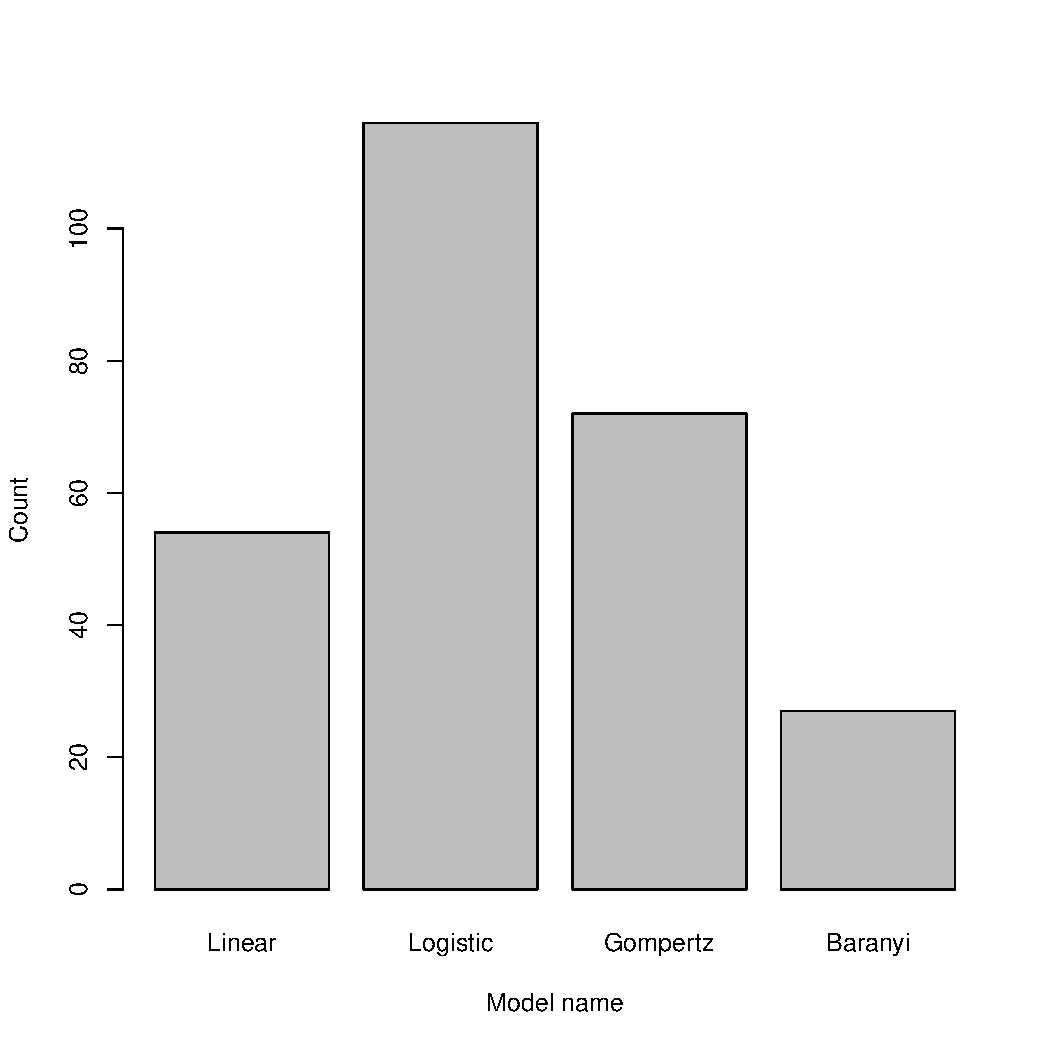
\includegraphics[keepaspectratio, width = 5in, height = 4in]{../results/lowAIC.pdf}
\centering
\caption{Bar chart showing the number of times {$\Delta$AIC} = 0 per model}
\end{figure}
\newpage
Comparison of the Akaike weights showed  that even though the classical mechanistic model had the largest {AIC\textsubscript{w}} overall, the median {AIC\textsubscript{w}} of the Gompertz model was slightly higher than that of the classical mechanistic model (Figure 3).

\begin{figure}[H]
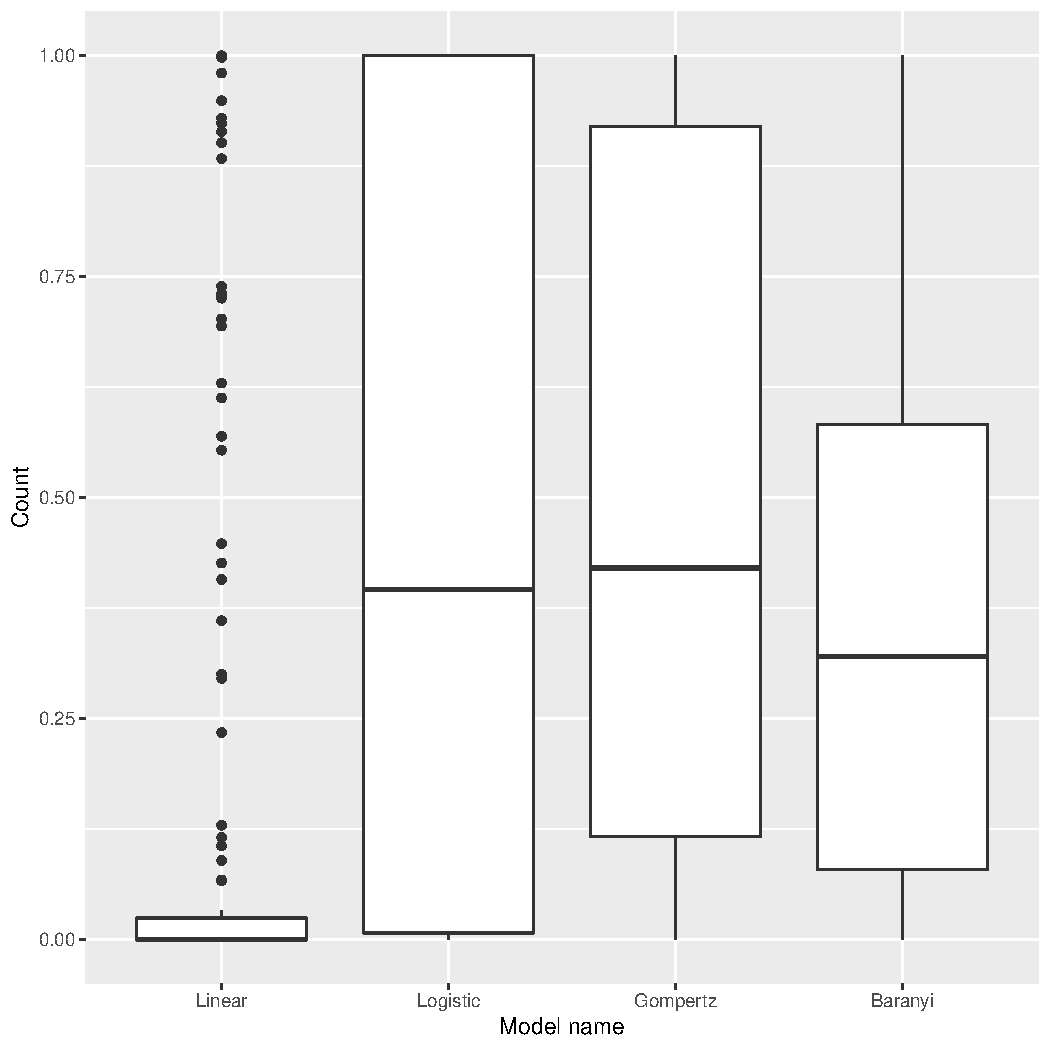
\includegraphics[keepaspectratio, width = 5in, height = 4in]{../results/aicw.pdf}
\centering
\caption{Box plot showing the distribution of {AIC\textsubscript{w}}}
\end{figure}
\newpage
Judging by the ratio of high {AIC\textsubscript{w}} relative to successful fits, Gompertz model and classical mechanistic model were very close, 0.49 compared to 0.48 (Figure 4).

\begin{figure}[H]
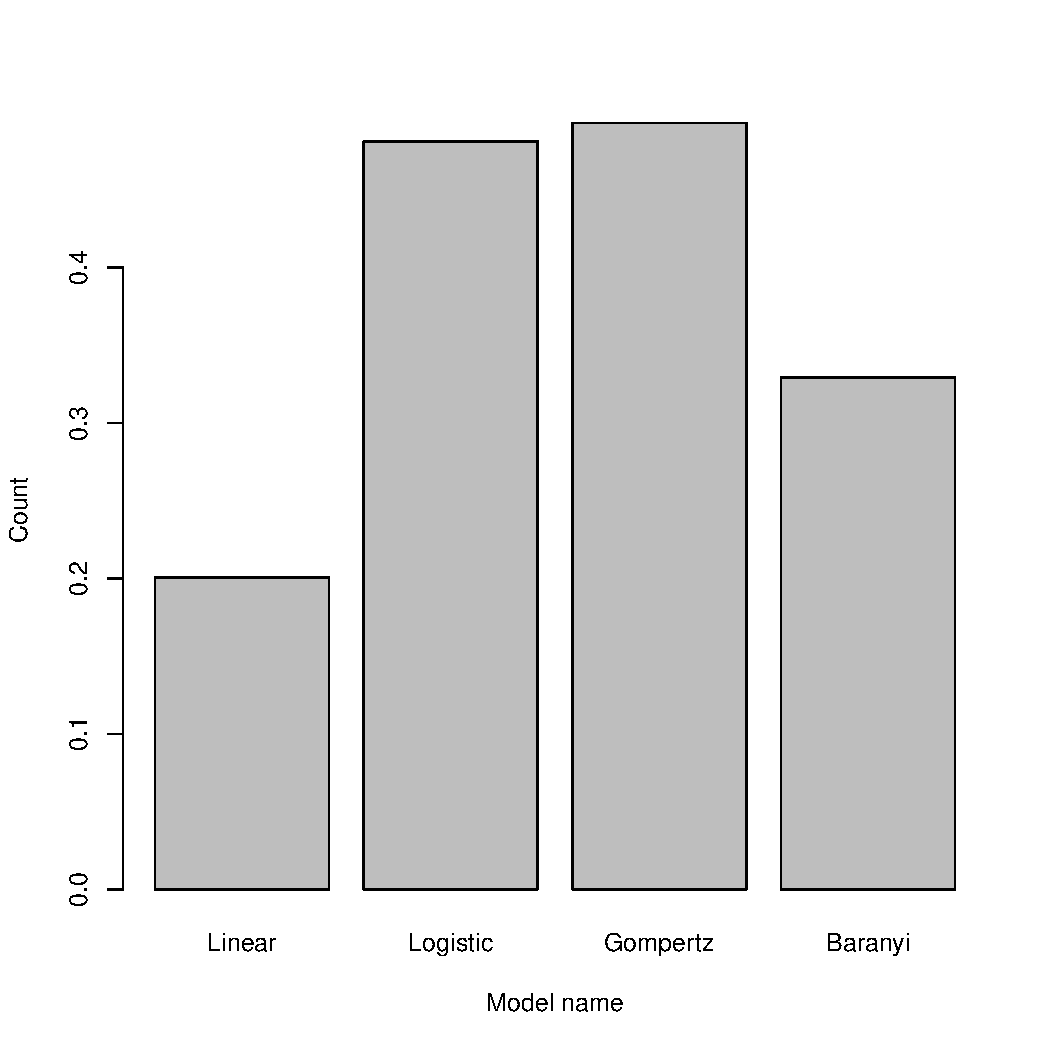
\includegraphics[keepaspectratio, width = 5in, height = 4in]{../results/ratio.pdf}
\centering
\caption{Bar chart showing the ratio of high {AIC\textsubscript{w}} to successful fits}
\end{figure}
\newpage
\section{Discussion}
The goal of this project is to identify the best fitting model from a group of four models which are linear growth, classical mechanistic, Gompertz, Baranyi. These models were fitted to the data and the goodness-of-fit was assessed through the Akaike Information Criterion. I conclude that the classical mechanistic model is the best model for the provided data. Despite the fact that the classical mechanistic model was only able to fit 43\% of the data, the evidence showed in figure 2 and figure 3 supports this claim. The classical mechanistic model has the highest count for the number of times {$\Delta$AIC} equals to 0 and the largest Akaike weights. Another model that exhibits great potential is the Gompertz model. Although the number of successful fits and the count of low {$\Delta$AIC} for the Gompertz model are not high, when assessing the Akaike weights among its successful fits, the values are quite comparable to that of the classical mechanistic model. The Baranyi model is a poor fit for these data, possibly due to the low number of data points in some sets. With a low count of data points, the \emph{r\textsubscript{max}} and \emph{t\textsubscript{lag}} could end up being too low, leading to the calculation of the extra parameter \emph{h} being not as accurate. The linear growth model has the best successful fit percentage, 100\% of the data were fitted to the linear. However, as expected, as the bacterial growth curve has three phases, a one-phase exponential linear growth model is a poor fit for these data. Therefore, the linear growth was only used to obtain the slope which was then used as the starting value for \emph{r\textsubscript{max}} in the non-linear regression models. 
\newpage
\section{Conclusion}
In conclusion, the classical mechanistic model is the best performing model. It is clear that the AIC favours models with fewer parameters as the classical mechanistic model outperformed both the Gompertz and the Baranyi model. Nonetheless, the Gomperzt model did show some promising results among its successful fits, the Akaike weight value of the Gompertz model was very close to that of the mechanistic models. I believe if the number of data points per unique set was more uniform, the Gompertz model would have performed better.

\newpage

\bibliographystyle{agsm}
\bibliography{bib}

\end{document}
